% $Id: report.tex 11 2007-04-03 22:25:53Z jpeltier $

\documentclass{vgtc}                          % final (conference style)
% \documentclass[onecolumn]{vgtc}             % one column
%\documentclass[review]{vgtc}                 % review
%\documentclass[widereview]{vgtc}             % wide-spaced review
%\documentclass[preprint]{vgtc}               % preprint
%\documentclass[electronic]{vgtc}             % electronic version

% Make references appear in order of appearance
\bibliographystyle{unsrt}

% Add page numbers
\makeatletter
\renewcommand{\@oddfoot}{\hfil\thepage\hfil}
\renewcommand{\@evenfoot}{\@oddfoot}
\makeatother

%% Uncomment one of the lines above depending on where your paper is
%% in the conference process. ``review'' and ``widereview'' are for review
%% submission, ``preprint'' is for pre-publication, and the final version
%% doesn't use a specific qualifier. Further, ``electronic'' includes
%% hyperreferences for more convenient online viewing.

%% Please use one of the ``review'' options in combination with the
%% assigned online id (see below) ONLY if your paper uses a double blind
%% review process. Some conferences, like IEEE Vis and InfoVis, have NOT
%% in the past.

%% Figures should be in CMYK or Grey scale format, otherwise, colour 
%% shifting may occur during the printing process.

%% These few lines make a distinction between latex and pdflatex calls and they
%% bring in essential packages for graphics and font handling.
%% Note that due to the \DeclareGraphicsExtensions{} call it is no longer necessary
%% to provide the the path and extension of a graphics file:
%% \includegraphics{diamondrule} is completely sufficient.
%%
\ifpdf%                                % if we use pdflatex
  \pdfoutput=1\relax                   % create PDFs from pdfLaTeX
  \pdfcompresslevel=9                  % PDF Compression
  \pdfoptionpdfminorversion=7          % create PDF 1.7
  \ExecuteOptions{pdftex}
  \usepackage{graphicx}                % allow us to embed graphics files
  \DeclareGraphicsExtensions{.pdf,.png,.jpg,.jpeg} % for pdflatex we expect .pdf, .png, or .jpg files
\else%                                 % else we use pure latex
  \ExecuteOptions{dvips}
  \usepackage{graphicx}                % allow us to embed graphics files
  \DeclareGraphicsExtensions{.eps}     % for pure latex we expect eps files
\fi%

%% it is recomended to use ``\autoref{sec:bla}'' instead of ``Fig.~\ref{sec:bla}''
\graphicspath{{figures/}{pictures/}{images/}{./}} % where to search for the images

\usepackage{microtype}                 % use micro-typography (slightly more compact, better to read)
\PassOptionsToPackage{warn}{textcomp}  % to address font issues with \textrightarrow
\usepackage{textcomp}                  % use better special symbols
\usepackage{mathptmx}                  % use matching math font
\usepackage{times}                     % we use Times as the main font
\renewcommand*\ttdefault{txtt}         % a nicer typewriter font
\usepackage{cite}                      % needed to automatically sort the references
%% We encourage the use of mathptmx for consistent usage of times font
%% throughout the proceedings. However, if you encounter conflicts
%% with other math-related packages, you may want to disable it.

\usepackage{makecell}
\usepackage{float}

%% If you are submitting a paper to a conference for review with a double
%% blind reviewing process, please replace the value ``0'' below with your
%% OnlineID. Otherwise, you may safely leave it at ``0''.
\onlineid{0}

%% declare the category of your paper, only shown in review mode
\vgtccategory{Research}

%% allow for this line if you want the electronic option to work properly
\vgtcinsertpkg

%% In preprint mode you may define your own headline.
%\preprinttext{To appear in an IEEE VGTC sponsored conference.}

%% Paper title.

\title{CityQuest - COMPSCI 732: Individual Report}

%% This is how authors are specified in the conference style

%% Author and Affiliation (single author).
%%\author{Roy G. Biv\thanks{e-mail: roy.g.biv@aol.com}}
%%\affiliation{\scriptsize Allied Widgets Research}

%% Author and Affiliation (multiple authors with single affiliations).
%%\author{Roy G. Biv\thanks{e-mail: roy.g.biv@aol.com} %
%%\and Ed Grimley\thanks{e-mail:ed.grimley@aol.com} %
%%\and Martha Stewart\thanks{e-mail:martha.stewart@marthastewart.com}}
%%\affiliation{\scriptsize Martha Stewart Enterprises \\ Microsoft Research}

%% Author and Affiliation (multiple authors with multiple affiliations)
\author{Romili Townsend \\ 
    \parbox{1.4in}{\scriptsize \centering University of Auckland}\\
    \parbox{1.4in}{\scriptsize \centering rtow454@aucklanduni.ac.nz}
}
%% Copyright space is enabled by default as required by guidelines.
%% It is disabled by the 'review' option or via the following command:
% \nocopyrightspace

%%%%%%%%%%%%%%%%%%%%%%%%%%%%%%%%%%%%%%%%%%%%%%%%%%%%%%%%%%%%%%%%
%%%%%%%%%%%%%%%%%%%%%% START OF THE PAPER %%%%%%%%%%%%%%%%%%%%%%
%%%%%%%%%%%%%%%%%%%%%%%%%%%%%%%%%%%%%%%%%%%%%%%%%%%%%%%%%%%%%%%%%

\begin{document}


%% The ``\maketitle'' command must be the first command after the
%% ``\begin{document}'' command. It prepares and prints the title block.
%% the only exception to this rule is the \firstsection command
\maketitle

\firstsection{}
\textbf{Abstract---CityQuest is a GPS-based mobile exploration game designed to encourage physical activity and improve users' familiarity with urban environments through navigation-based tasks.
The system assigns challenges at locations within the city that users must travel to in order to complete. Gamification elements such as streaks, levels, badges, and leaderboards are employed to increase user motivation and engagement.
This report outlines the motivation, design, and implementation of this system developed for the COMPSCI 732 course, and compares it to existing solutions.}

%% \section{Introduction} %for journal use above \firstsection{..} instead

\section{Introduction} 

Less than half of the New Zealand population meets recommended physical activity guidelines \cite{PhysicalActivityProfilesandPerceivedEnvironmentalDeterminantsinNewZealandANationalCrossSectionalStudy}. This highlights the need for interventions that encourage greater participation in physical activity and increase user engagement.

A systematic review and meta-analysis found that gamification interventions are effective at promoting physical activity across diverse age groups and genders and may outperform alternative interventions \cite{mazeas2022gamification}. Gamification therefore presents a promising approach for encouraging physical activity while maintaining user motivation and engagement.

Beyond physical activity, environmental interaction may influence how people learn to navigate their surroundings. Environmental familiarity has been associated with improved wayfinding performance, including reduced navigation errors and shorter route completion times \cite{ONEILL1992319}. In addition, repeated exposure to an environment has been shown to support the acquisition of spatial knowledge in multiple dimensions, including landmark recognition and route learning \cite{YING2026103031}. Together, these findings suggest that increasing familiarity with local environments may improve users' navigation ability through the development of stronger spatial knowledge.

This project addresses both objectives by employing gamified, navigation-based activities that promote exploration and interaction with local environments, with the aim of increasing environmental familiarity and physical activity levels.

\section{Goals}

Create a GPS-based city exploration game that rewards movement and exploration of the local environment.

\begin{itemize}
    \item Encourage physical activity through gameplay that requires movement, reinforced by reward-based incentives.
    \item Promote environmental familiarity through interaction with local landmarks and points of interest.
    \item Promote an engaging, gamified alternative to traditional navigation tools.
\end{itemize}

\section{Related Work}

Several existing solutions incorporate location-based interaction and exploration-based gameplay. Notable examples include \textit{Pokemon Go}\cite{pokemon_go} and \textit{Ingress}\cite{ingress}, both of which use GPS-backed movement as a core gameplay mechanic to encourage real-world exploration and physical activity.  

While these location-based games require users to physically travel to geographic locations, interaction with these environments is primarily mediated through game mechanics rather than direct engagement with the world. In these systems, players interact with virtual elements overlaid on geographic locations, such as collecting items or capturing creatures.

In contrast, this project requires users to engage directly with the physical environment through curated, contextually relevant real-world tasks. Unlike existing systems, the primary interaction occurs within the physical environment rather than within the application itself.

In the domain of navigation, Google Maps\cite{google_maps} is a widely used application that supports local discovery and route planning. Features such as \textit{Search This Area} allow users to explore points of interest within a geographic region, including categories such as restaurants and parks. Location discovery is further supported through filtering based on various criteria, such as proximity, user ratings, and popularity. The platform also provides optimised route planning through turn-by-turn navigation instructions, prioritising minimising travel time.

While these features support navigation and location discovery, Google Maps is designed primarily to optimise travel efficiency by identifying the fastest route to a location rather than encourage physical activity and exploration. In Google Maps, users typically specify a destination first and are subsequently guided there.

In contrast, CityQuest provides users with daily, location-backed challenges that encourage exploration, environmental interaction, and physical activity. In addition, CityQuest incorporates game mechanics to encourage exploration and movement, whereas Google Maps does not.

\section{Design}

We created an ERD with PlantUML during the initial system planning phase to visualise the relationships between entities within the system. As the system evolved, we updated this ERD to reflect the changes in the system. This final ERD can be see in Figure~\ref{fig:erd}.

As can be seen in the ERD, there is an inherent relationship between each entity type in the database. For example, users are assigned user challenges, each of which corresponds to a challenge, and each of which which has an associated category. This highly related nature of the entities in our data influenced our decision in choosing a relational database such as PostgreSQL over a document-oriented database such as MongoDB.

\subsection{Tech Stack}
\subsection{Backend}
\begin{itemize}
    \item \textbf{Prisma} was used as an ORM to provide type-safe access to the database and simplify code by minimising having to write complex SQL queries. Its generated TypeScript files improve developer productivity by enabling autocompletion.
    \item \textbf{Supabase Auth} was used to handle user authentication and account management. This was chosen for its simple integration into the Supabase ecosystem, and because it is a widely used, secure authentication service so reduces security risks compared to developing a custom authentication service from scratch.
    \item \textbf{Google OAuth} was chosen to provide a convenient, secure sign-in method. By allowing users to sign-in with an existing Google account, the registration process is faster. Furthermore, using a passwordless sign-in option means there is no risk of the user's password being exposed in the event of a data breach as we do not store any passwords.
    \item \textbf{Express} was used to implement the application's API layer. Express was chosen because it is lightweight and accelerates development through hot reloading, where the API server restarts itself when it detects changes made in development. The Express API server handles the business logic, routing, and communication between the frontend web server and backend database.
    \item \textbf{TypeScript} was used to extend JavaScript to support type safety, catching type errors and allowing for IDE auto completion and suggestions.
\end{itemize}

\subsection{Frontend}
\begin{itemize}
    \item \textbf{React} was chosen for building the user interface due to its component-based architecture. When the application state changes, React efficiently updates only the effected UI components rather than reloading the entire page.
    \item \textbf{Vite} was chosen as the build tool for React as it offers a fast development server, hot reloading on changes, and a simple build process for easy deployment.
    \item \textbf{TypeScript}
\end{itemize}

\subsection{User Interface}
Low-fidelity Figma mockups were created for the Challenge list, challenge map, achievements, and profile pages of the frontend system user interface, as can be see in Figures~\ref{fig:mockup-1} and~\ref{fig:mockup-2}. These prototypes were created to serve as inspiration for the in-development system, identify early and UX concerns, and ensure all group members had a consistent vision for the system.

\begin{figure}[htbp]
    \centering
    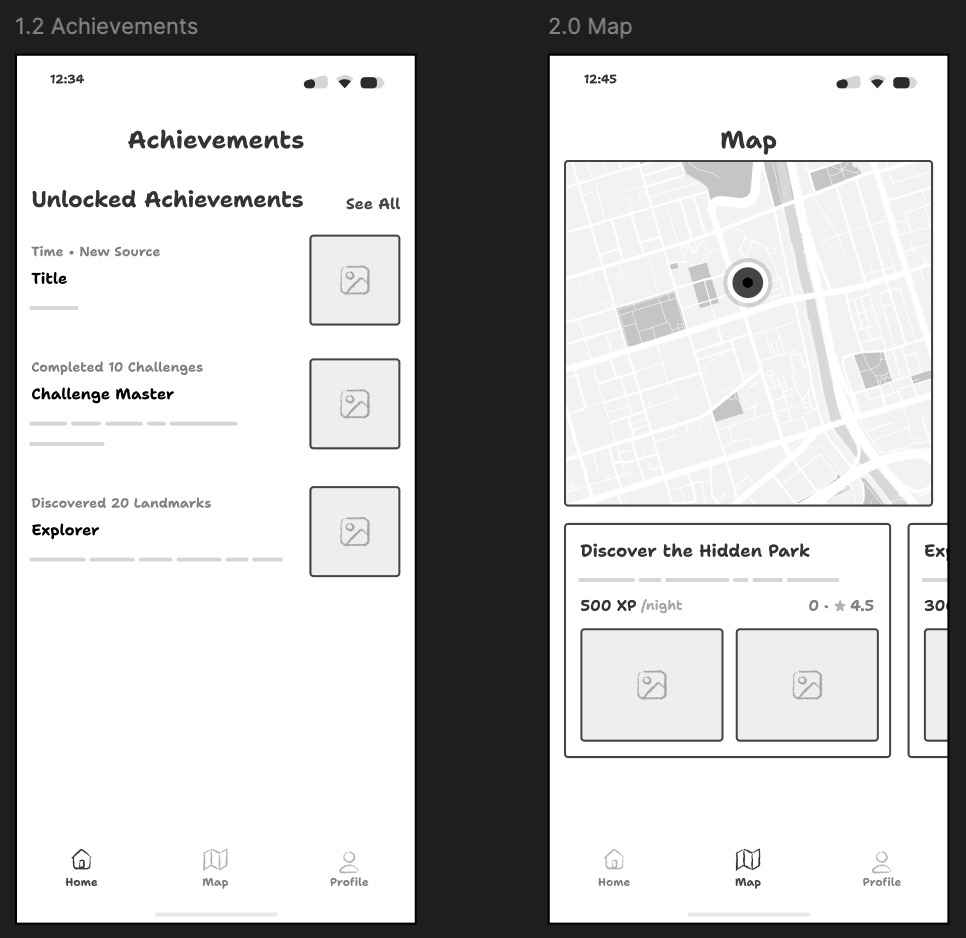
\includegraphics[width=0.9\linewidth]{Figma-1.png}
    \caption{Figma mockups of the Achievements and Map view pages}
    \label{fig:mockup-1}
\end{figure}

\begin{figure}[htbp]
    \centering
    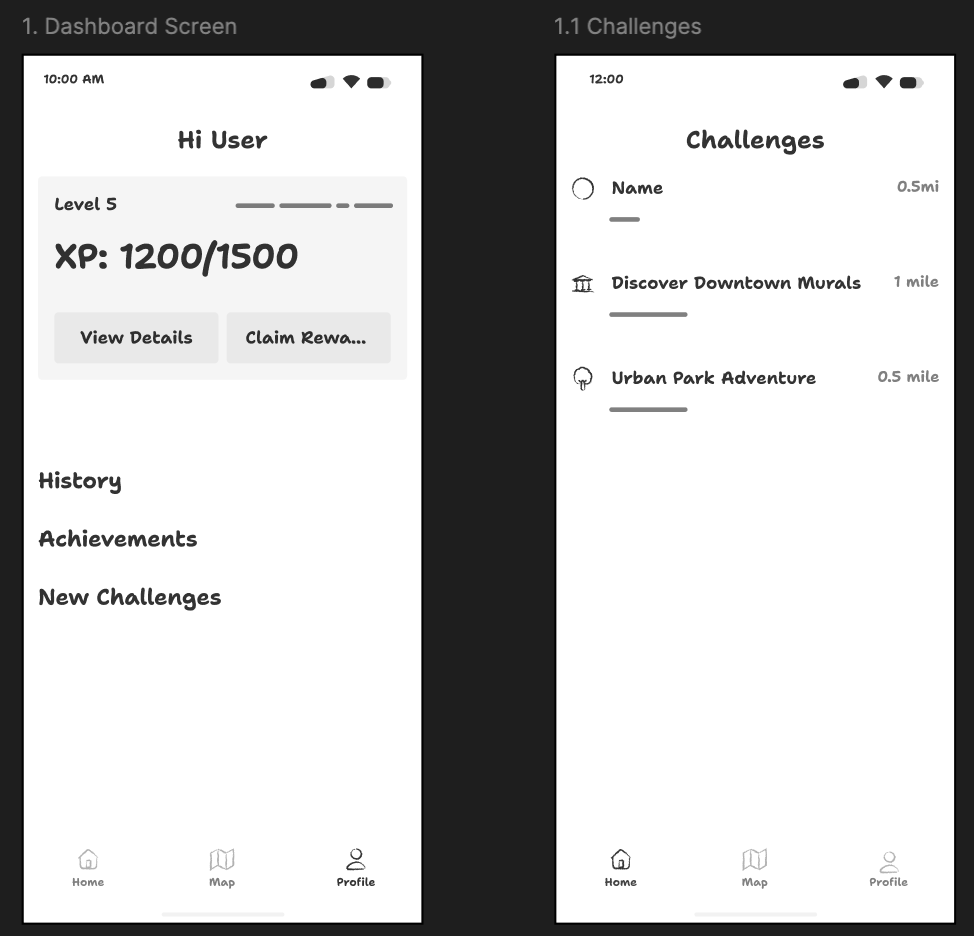
\includegraphics[width=0.9\linewidth]{Figma-2.png}
    \caption{Figma mockups of the Profile and Challenge view pages}
    \label{fig:mockup-2}
\end{figure}

\section{Implementation: What have you implemented?}

The system implements a location-based challenge workflow. The sequence diagram in Figure~\ref{fig:sequence-diagram} outlines the full interaction flow between the user, frontend web server, backend API and database, and external services.

When a user opens the application and navigates to the challenge list page, they are presented with a list of nearby, available daily challenges retrieved from the backend. These challenges include metadata such as category (e.g. fitness, social, nature) and location (e.g. a nearby park or restaurant). The user can then select and accept a challenge.

After accepting a challenge, the user can click the \textit{View Route} button which displays a focused map view displaying the user's current location, the challenge location marker, and the router between them. This allows the user to navigate to the challenge location.

Once the user arrives at the location, they perform a check-in by pressing the \textit{Check-In} button on the active challenge view. This triggers the frontend to send the user's current location to the backend API, where it is validated to ensure the user is within the required geospatial proximity. If validation is successful, the challenge is marked as complete in the backend database.

Completion of a challenge triggers several backend updates, including awarding experience points, recalculating the user's level, updating the user's daily streak, and user statistics. When the \texttt{user\_stats} table is updated, a PostgreSQL trigger evaluates the badge criteria table to determine whether any badge requirements have been satisfied. If all criteria for a badge are met, the badge is awarded to the user.

Finally, the backend passes the updated experience, level and badge information to the frontend. The user interface displays a celebratory confetti animation, notifications for any newly earned badges, and an updated experience progress bar animation.

\begin{figure}[htbp]
    \centering
    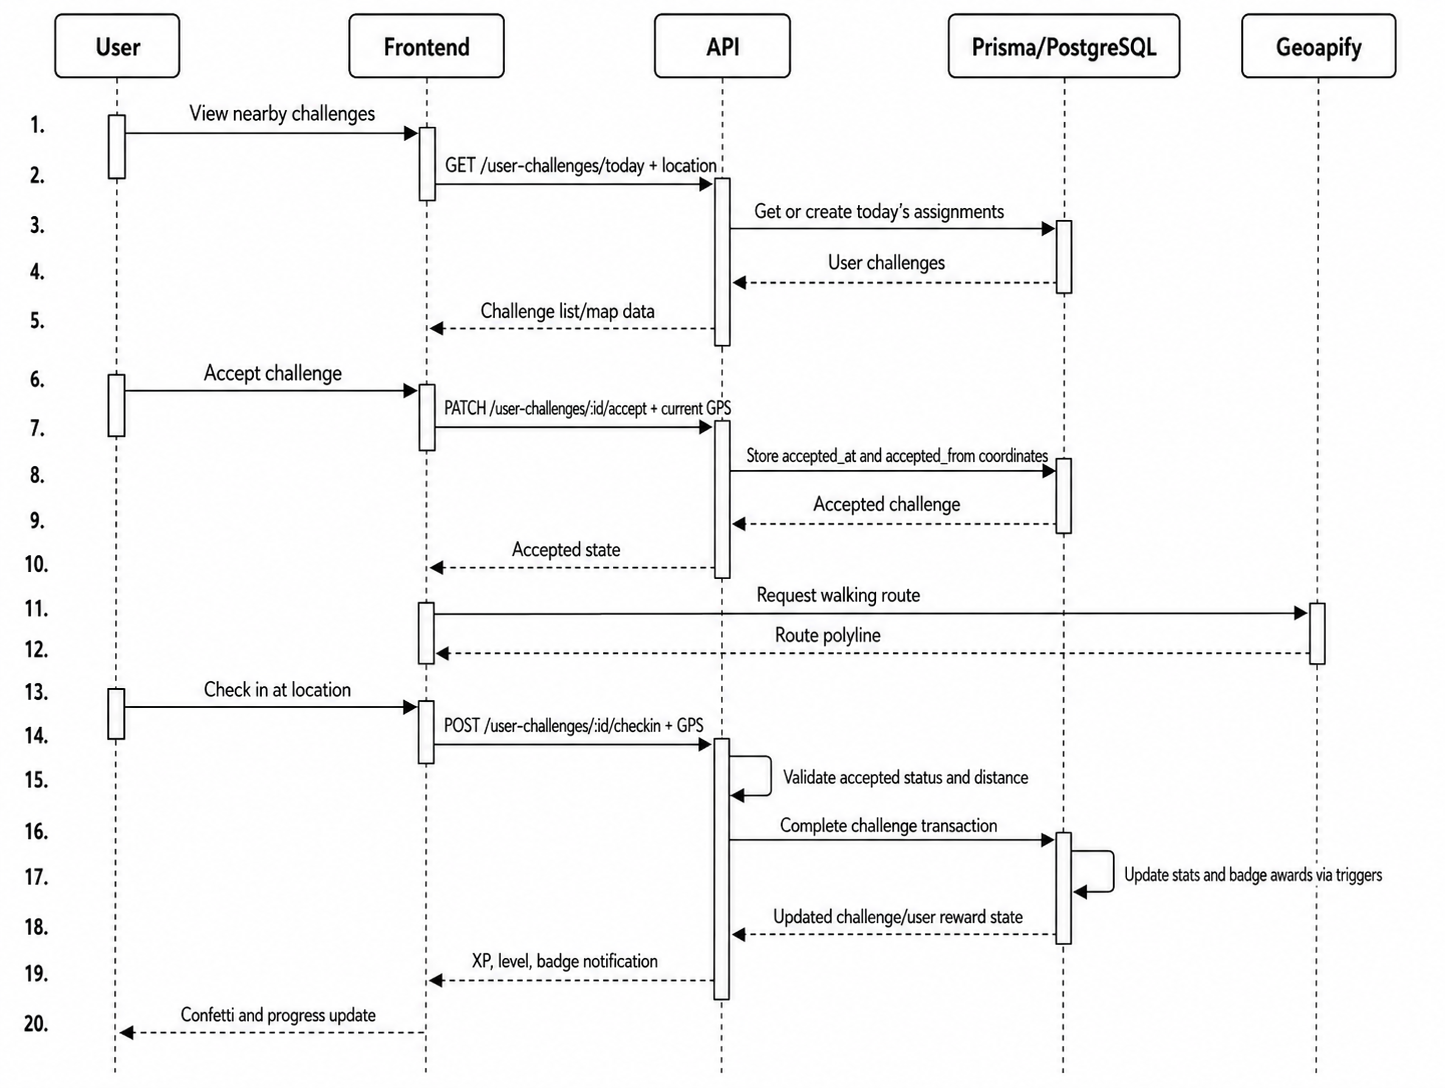
\includegraphics[width=0.9\linewidth]{pictures/sequence-diagram.png}
    \caption{Sequence diagram for the challenge participation workflow}
    \label{fig:sequence-diagram}
\end{figure}

\subsection{Deployment}
The frontend was deployed as a Single Page Application (SPA) using Vercel's free tier. Vercel integrates with GitHub to automatically build and deploy the frontend whenever commits are pushed to configured branches, enabling a rapid deployment workflow.

Supabase was used to host the PostgreSQL database and provide authentication services.
The API server, which communicates with the database, was deployed as a Render web service using the free tier. Similar to the Vercel frontend deployment, Render integrates with GitHub and automatically builds and deploys the API server whenever commits are pushed to configured branches.

One limitation of this deployment method is that Render's free tier service automatically spins down after 15 minutes of inactivity. When the service has spun down, the first request experiences a cold-start delay and times out while the service restarts. This startup process typically takes approximately one minute before the API becomes responsive to requests again.

\section{Testing}

Backend testing was performed using Vitest. Unit tests were used to verify the functionality of individual components, while integration tests validated the database interactions, schema constraints, and trigger functionality.
Supertest was used to test API endpoints by simulating HTTP requests and verifying that the correct response status codes and response bodies were returned.
Additionally, TypeScript type checking was used to detect static typing errors during development.

Frontend component testing was performed using Vitest and React Testing Library. These tests verified component rendering, user interactions, and application state changes within a simulated browser environment provided by jsdom.

End-to-end testing was performed using Playwright. These tests validated user workflows by simulating user interactions with the application through a web browser, ensuring that the frontend and backend component functioned correctly when integrated into the overall system. The end-to-end test suite was incorporated into the GitHub Actions CI/CD pipeline to automatically execute on every commit, providing continuous verification of the application's functionality.

One limitation of the testing suite is a lack of code test coverage analysis. While the unit, integration, and end-to-end tests provide functionality assurances across many components of both the backend and frontend codebases, there is no coverage testing set up to measure how much of the source code is executed during testing. As a result, there may be hidden bugs in these areas of the codebase that are not detected from running the test suite. 
For the purpose of this report, test coverage analysis with Vitest was conducted for the frontend and backend codebases, the results of which are summarised in Table~\ref{tab:coverage-tests}. Full results can be found in the Figures~\ref{fig:frontend-coverage} and~\ref{fig:backend-coverage} within the Appendix.

\begin{table}[htbp]
    \centering
    \begin{tabular}{|c|c|c|c|c|}
        \hline
        \makecell{Module} & 
        \makecell{Statement\\Coverage} &
        \makecell{Branch\\Coverage} &
        \makecell{Functions\\Coverage} &
        \makecell{Line\\Coverage} \\
        \hline
        Frontend & 79.14\% & 70.16\% & 77.3\% & 82.1\% \\
        Backend & 73.65\% & 61.22\% & 67.11\% & 74.02\% \\
        \hline
    \end{tabular}
    \caption{Frontend Test Coverage by Codebase}
    \label{tab:coverage-tests}
\end{table}

As can be seen in the Table~\ref{tab:coverage-tests} and Figures~\ref{fig:frontend-coverage} and~\ref{fig:backend-coverage}, the frontend achieves higher coverage than the backend in all metrics. This suggests that frontend components are tested more thoroughly by the test suite. The most significant gap missed by the test suite is the Domain Access Objects (DAOs), with a branch coverage of 0\%.

\section{Methodology}

The project adopted an iterative, sprint-based development cycle based on Agile methodologies. Work was organised into weekly sprints. At the beginning of each sprint, tasks were defined, prioritised, and allocated to individual team members. To reduce ambiguity in task completion, each task included clearly defined acceptance criteria specifying what conditions needed to be met for the task to be considered complete.

The team held weekly sprint meetings to coordinate development and check-in on each member's progress. During these meetings, attendance was recorded and discussions were documented in meeting minutes for future reference. If any team member was absent, they were briefed via the team Discord server and could refer to the full meeting minutes for further information. Meeting times were scheduled each week based on the overlapping availability of all team members, collected using the scheduling tool Timeful, to maximise attendance. Due to inconsistent team member availability and differing amounts of discussion required each week, the scheduled duration of meetings varied from week to week, and meetings were flexibly adjusted to accommodate these factors.

Task prioritisation was managed using the MoSCoW method, categorising work into Must have, Should have, Could have, and Won't have (out of current scope) requirements, ordered from highest to lowest priority.

For each task that we created, we added a corresponding issue ticket to GitHub. Commits referenced these issues so that team members could easily trace changes back to specific commits. Tasks were organised and tracked using a Github Projects Kanban board which provided a visual representation of the progress of the project and current sprint. Table~\ref{tab:kanban} outlines the different Kanban board task categories and their status.

\begin{table}[htbp]
    \centering
    \begin{tabular}{|c|c|}
        \hline
        Category & 
        Task Status \\
        \hline
        Product Backlog & Not yet assigned to a sprint \\
        To Be Decided & Not yet assigned to a team member \\
        Sprint Backlog & Part of the active sprint but not started \\
        In Progress & Actively being worked on \\
        In Review & Completed pending pull request approval \\
        Done & Completed \\
        \hline
    \end{tabular}
    \caption{Kanban board categories}
    \label{tab:kanban}
\end{table}

During the "In Review" stage, if a pull request was rejected, then the task would be moved backwards to the "In Progress" status and then later moved forward to "In Review" again upon the requested changes being made.

Changes were made in sub-branches of the \textit{feature} and \textit{bug} branches. Upon a feature being completed, a pull request was made to bring those changes to the main branch, with the related issues being referenced in the pull request message. This was done to ensure the main branch only contained completed, tested features. All pull requests were peer reviewed by at least one other team member before being merged into the main branch, ensuring code quality and consistency.

In addition, a Discord webhook was configured to automatically notify the team when new pull requests were created, updated, or merged. This helped keep everyone informed of ongoing changes and improved visibility of development activity without requiring constant manual checking of GitHub.

\section{Tooling}

Generative AI was used by some team members to increase efficiency, particularly for menial tasks where the code is easy to validate. 

Copilot code review was used in multiple instances to check for any bugs, syntax errors, and suggest considerations. However, this was not used as a substitute to human-run peer reviews but rather in addition to; all pull requests to the main branch were peer reviewed by at least one other team member.

Git and GitHub were used throughout development for version control and collaboration. The use of feature branches and pull requests allowed team members to work independently and minimise merge conflicts while ensuring stability of the main branch. 

Git and GitHub was used frequently throughout the development process for version control and collaboration. Feature branches enabled team members to develop features independently while reducing the risk of introducing unstable code into the main branch. GitHub's pull request system supported peer reviews and discussion before changes were merged to main.

While Git was highly effective overall, its use came with some difficulties. In two separate instances, contributors accidentally pushed commits directly to the main branch rather than through the pull request process, unintentionally bypassing the intended review process. Team members also occasionally made commits using incorrect Git email addresses due to configuration issues, resulting in some team members' contributions being split between their alternate accounts. Despite these challenges, the Git version control system was very effective in supporting collaborative development.

\section{Discussion: Have the goals been achieved? Problems?}

A user study could be valuable to investigate whether this city exploration game had an impact on users' familiarity with their surroundings, and whether it increased users' physical activity levels, particularly average daily step counts. Unfortunately, due to the nature of the course, it was not feasible to conduct a user study.

In our project proposal we marked 13 tasks as must haves, 6 tasks as should haves, 10 tasks as could haves, and 4 tasks as out of scope.
Of these tasks, all must haves were completed, all should haves, 2 could haves, and no out of scope tasks.

The following table compares, for every prioritisation category, the number of tasks completed vs the number of tasks assigned.

\begin{table}[htbp]
    \centering
    \begin{tabular}{|c|c|c|c|}
        \hline
        Prioritisation & 
        \makecell{Completed\\tasks} & 
        \makecell{Assigned\\tasks} & 
        \makecell{Percent\\completed} \\
        \hline
        Must have & 13 & 13 & 100\% \\
        Should have & 6 & 6 & 100\% \\
        Could have & 2 & 10 & 20\% \\
        \hline
        Total (within scope)& 22 & 29 & 75.86\% \\
        \hline
        Won't have (outside scope)& 0 & 4 & 0\% \\
        \hline
    \end{tabular}
    \caption{Task completion summary by prioritisation category}
    \label{tab:completion_summary}
\end{table}

\section{Conclusion: Conclusions? Lessons learned? Reflections? Future work?}

\subsection{Lessons Learned}


\subsection{Future Work}
While all the core functionality of our application was met, the project can be improved to boost the engagement of users and become more accessible.

One area of future work is improving the accessibility of CityQuest for users with disabilities. The current system does not include accessibility settings or provide accessibility information for challenges. CityQuest also assumes that users are able to physically travel to and interact with locations in the environment, which may exclude individuals with mobility impairments.

Future iterations of the system should introduce adjustable movement requirements, allowing users with limited mobility to be assigned challenges of a shorter travel distance. Additionally, the system could incorporate accessible route generation and provide accessibility information for each challenge location to better support participation among a diverse user base.

\section{Appendix}

\begin{figure}[H]
    \centering
    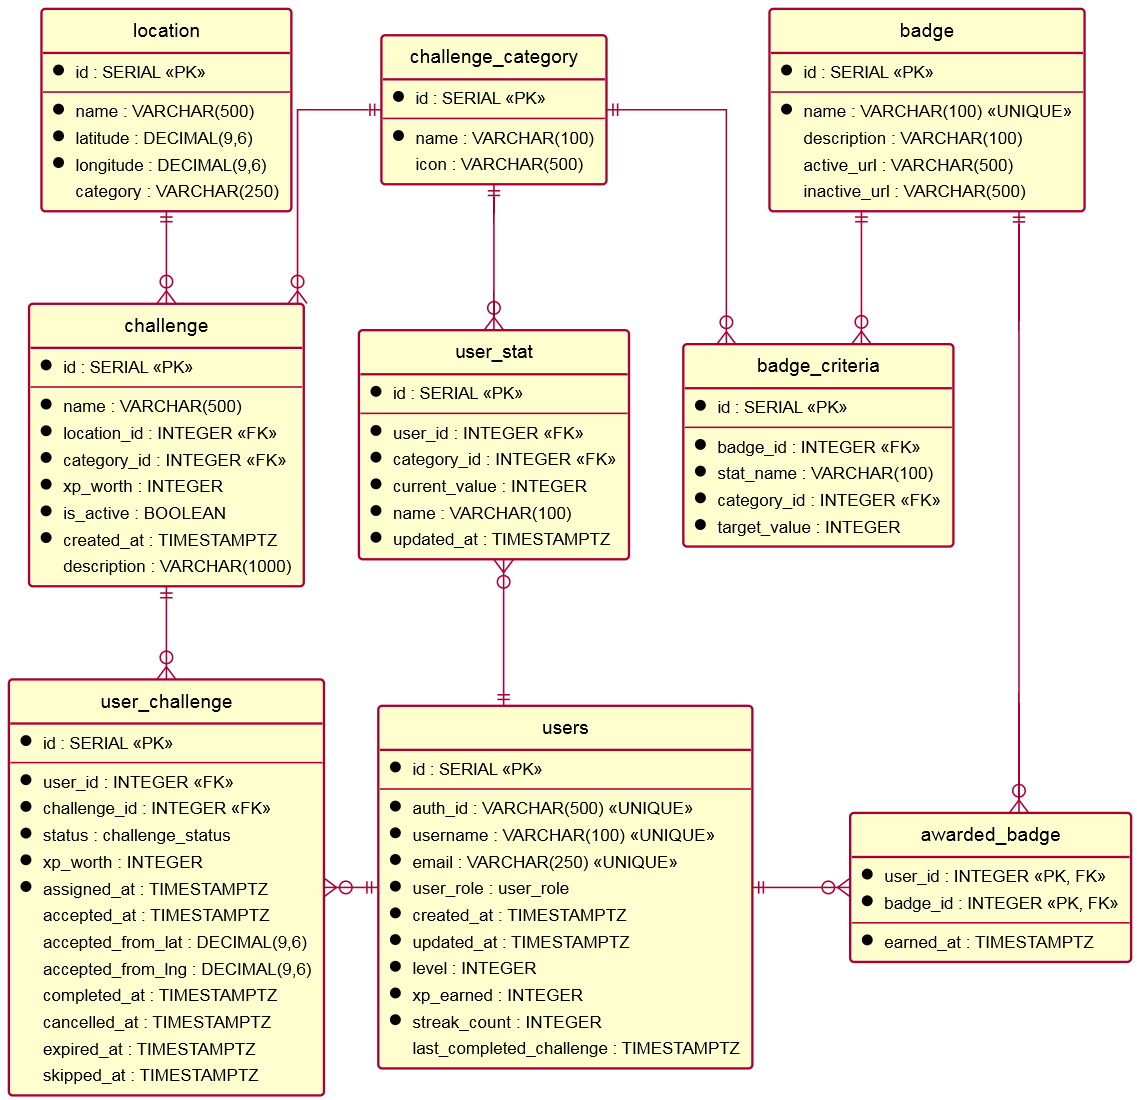
\includegraphics[width=1.05\linewidth]{pictures/erd.png}
    \caption{Entity Relationship Diagram of the CityQuest project}
    \label{fig:erd}
\end{figure}

\begin{figure}[H]
    \centering
    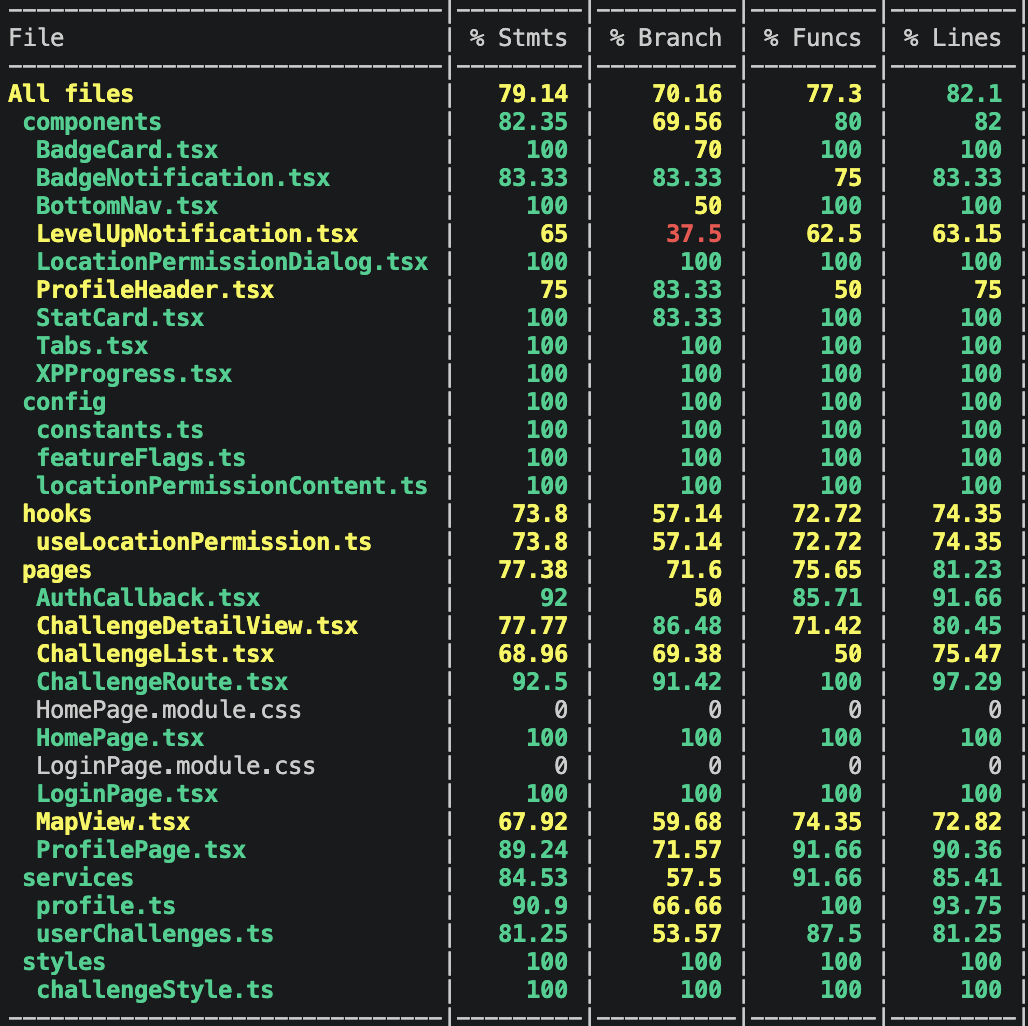
\includegraphics[width=0.95\linewidth]{pictures/Frontend-Coverage.png}
    \caption{Frontend Coverage Analysis Results}
    \label{fig:frontend-coverage}
\end{figure}

\begin{figure}[H]
    \centering
    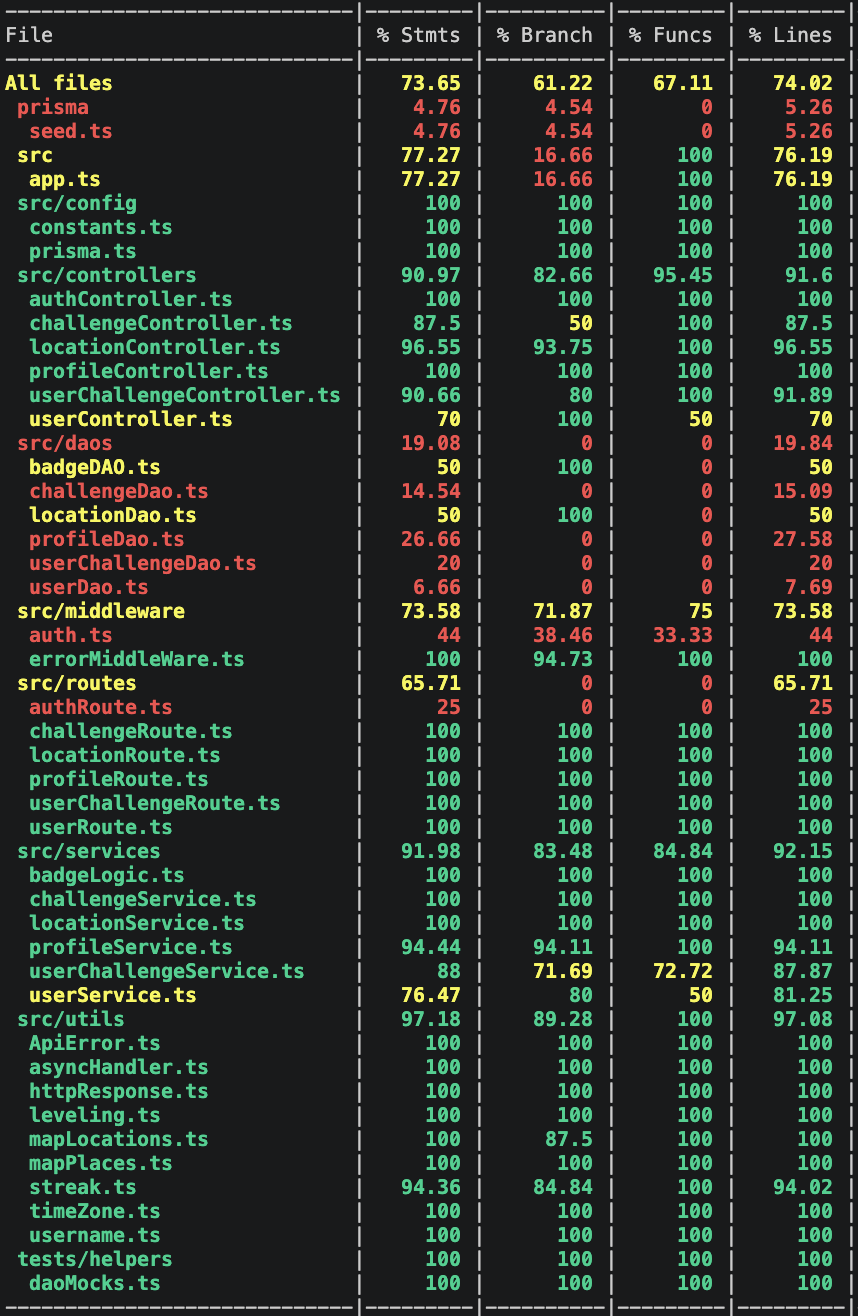
\includegraphics[width=0.95\linewidth]{pictures/Backend-Coverage.png}
    \caption{Backend Coverage Analysis Results}
    \label{fig:backend-coverage}
\end{figure}

\begin{figure*}[t]
    \centering
    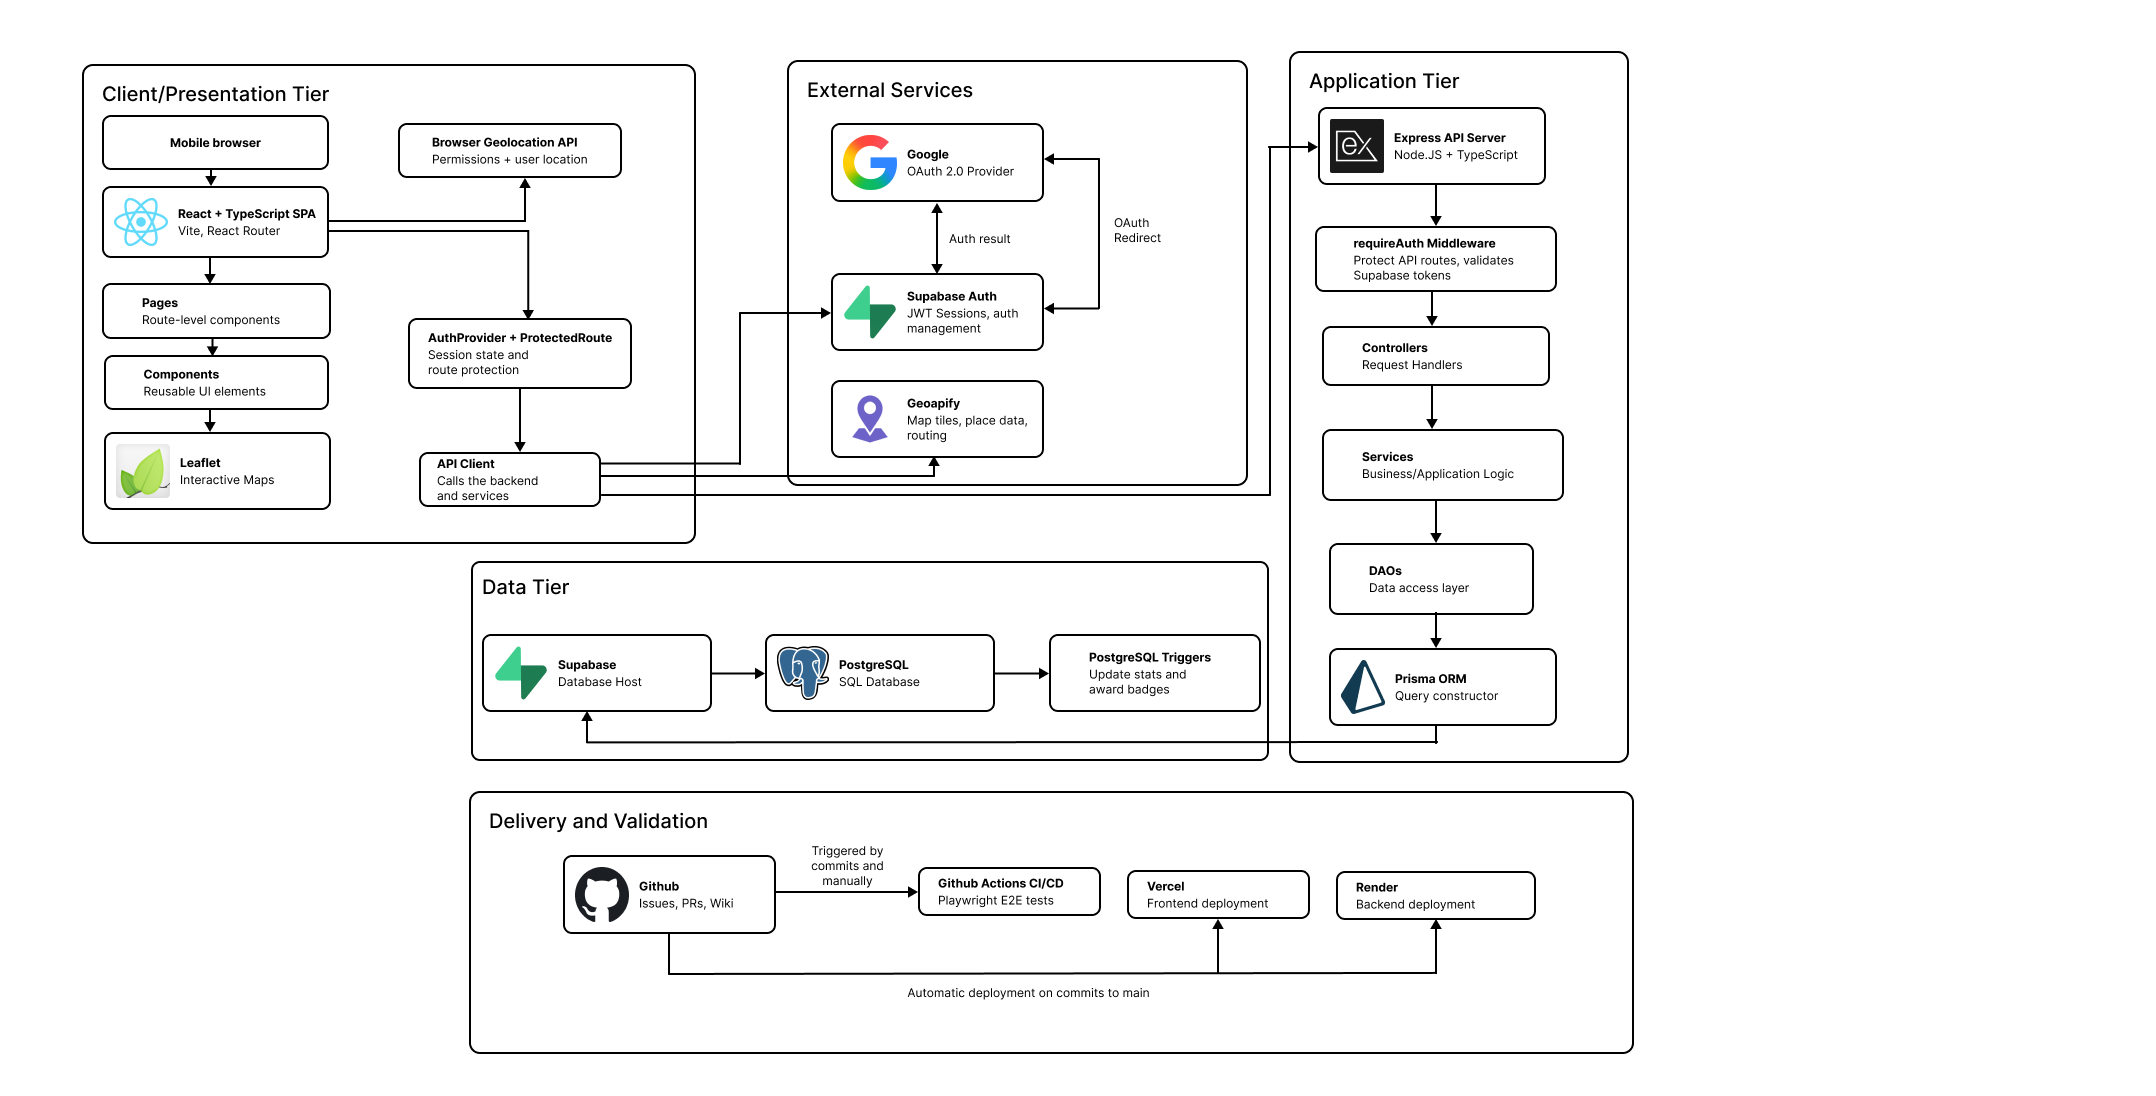
\includegraphics[width=1\linewidth]{system-architecture.png}
    \caption{Full-stack system architecture diagram}
    \label{fig:system-architecture}
\end{figure*}

%\bibliographystyle{abbrv}
\bibliographystyle{abbrv-doi}
%\bibliographystyle{abbrv-doi-narrow}
%\bibliographystyle{abbrv-doi-hyperref}
%\bibliographystyle{abbrv-doi-hyperref-narrow}

\bibliography{references}

\end{document}